\RequirePackage{silence}
\WarningFilter{hyperref}{Token not allowed}
\WarningFilter{microtype}{tracking amount}
\WarningFilter{chessfss}{\comment already}

% Transparency mode (no overlays)
\documentclass[xcolor={x11names,svgnames,dvipsnames},trans]{beamer}

\usepackage{pgfpages}
\usepackage{subfig}
\usepackage{tikz}
\usetikzlibrary{arrows,shapes,positioning,shadows,trees}

\usepackage[british]{babel}

%% Glossy pretty look for the presentation and transparency (w/o overlays and animations) versions!
\mode<beamer|trans>{
\useoutertheme[glossy]{wuerzburg}
\useinnertheme[shadow,outline]{chamfered}
\usecolortheme{shark}
}
\setbeamertemplate{navigation symbols}{}
\setbeamertemplate{frametitle continuation}[from second][(cont'd)]
\usefonttheme[stillsansseriftext,stillsansserifsmall]{serif}

%% Save up on ink for the 4-up handouts
\mode<handout>{
\useoutertheme{wuerzburg}
\useinnertheme[outline]{chamfered}
%\pgfpagesuselayout{4 on 1}[a4paper, landscape, border shrink=10mm]
\pgfpagesuselayout{2 on 1}[a4paper, border shrink=10mm]
\pgfpageslogicalpageoptions{1}{border code=\pgfstroke}
\pgfpageslogicalpageoptions{2}{border code=\pgfstroke}
\setbeamercolor{structure}{fg=black}
\setbeamercolor{alerted text}{fg=black}
}

\mode<presentation>{\AtBeginSection[]{%
\begin{frame}
\frametitle{Contents}
\tableofcontents[currentsection]
\end{frame}}}

\usepackage[T1,safe]{tipa}
\usepackage{microtype}
\usepackage[utf8]{inputenc}
\usepackage[T1]{fontenc}
\usepackage{libertine}
\usepackage[scaled=.77]{beramono}
\SetTracking{encoding=*}{-39}

\usepackage{relsize,tabularx}
\usepackage{hologo,textcomp}
\usepackage{multicol,booktabs}
\usepackage{listings}
\lstset{upquote,keepspaces=true,columns=spaceflexible,
basicstyle=\ttfamily\scriptsize,%
breaklines=true,breakindent=0pt,xleftmargin=0pt, xrightmargin=6pt,%
language=[LaTeX]TeX, texcsstyle=*\bfseries\color{Maroon}, commentstyle=\sffamily\itshape\smaller\color{SeaGreen4},
emphstyle=\bfseries\color{RoyalBlue3},escapechar={:},
emphstyle={[2]{\bfseries\color{Sienna2}}},
postbreak=\mbox{{\smaller\color{gray}$\hookrightarrow$}}
}

\mode<handout>{
   \lstset{
   texcsstyle=*\bfseries, commentstyle=\sffamily\itshape\smaller,
   emphstyle=\bfseries,escapechar={:},
   emphstyle={[2]{\bfseries}},
   emphstyle={[3]{\bfseries}},
   postbreak=\mbox{{\smaller$\hookrightarrow$}}
   }
}

\makeatletter
\lst@CCPutMacro\lst@ProcessOther {"2D}{\lst@ttfamily{-{}}{-{}}}
\@empty\z@\@empty
\makeatother


\usepackage{pgfgantt}
\usetikzlibrary{backgrounds}

\usepackage{multicol,multirow}
\usepackage[version=3]{mhchem}
\usepackage{expex,qtree}
\usepackage[detect-all]{siunitx}
\usepackage[siunitx]{circuitikz}
\usepackage{smartdiagram}
\usepackage{bytefield}
\usepackage{pgfplots}
\pgfplotsset{compat=1.12}
\usepackage{gchords,guitar}
\usepackage{spreadtab}
\usepackage{ccicons}
\usepackage{marvosym}
\usepackage{upgreek}
\usepackage{adforn}
% \ifpdf
\pdfmapfile{+webo.map}
% \fi
\newcommand{\wb}[1]{{\usefont{U}{webo}{xl}{n}#1}}
\usepackage{bookmark}

\setlength\fboxsep{0pt}

\author[Mubashir Hanif\\, Ahmad Sakor\\, Omar Gutiérrez]{\texorpdfstring{Mubashir Hanif,\\ Ahmad Sakor,\\ Omar Gutiérrez}{Mubashir Hanif, Ahmad, Omar Gutiérrez}}
\title{Image Processing}
\subtitle{\texorpdfstring{\textsc{Project 3: Interpolation and Image Warping}\\%
\hrulefill\ \adforn{57}\thickspace\thickspace\adforn{29}\ \hrulefill}{}}
\date[\ccbyncsa]{\ccbyncsa}

%\titlegraphic{\includegraphics[width=.3\textwidth]{TFZsuperellipse-crop}\\\tiny Illustration by Duane Bibby}

\hypersetup{%
pdfauthor={Omar Gutiérrez},
pdfkeywords={Image Processing}
}

\begin{document}
\begin{frame}[plain]
\maketitle
\end{frame}

\begin{frame} \frametitle{Contents}
    \tableofcontents
\end{frame}

%-=-=-=-=-=-=-=-=-=-=-=-=-=-=-=-=-=-=-=-=-=-=-=-=
% SECTION: Radial Basis Function
%-=-=-=-=-=-=-=-=-=-=-=-=-=-=-=-=-=-=-=-=-=-=-=-=

\section{Radial Basis Function}
\subsection{Radial Basis Function Interpolation}
\begin{frame}{Radial Basis Function Interpolation}
    \begin{itemize}
        \item We are using a Gaussian solution, but, there are other different option:
            \begin{itemize}
                \item Multiquadratic (most common, by default in Scipy)
                \item Inverse multiquadratic
                \item Thin-plate spine
            \end{itemize}
        \item We are reconstructing \textit{unknown functions} from \textit{known data}.
        \item Here, we look for weights $w_i$ 
        \item The solution is: $w = \phi^{-1} \cdot y$
        \item $y$ is the vector of values we want to \textit{learn}
    \end{itemize}
\end{frame}

\begin{frame}{Comparison with Scipy implementation}
    \begin{center}
        \begin{figure}
            \includegraphics[height=6.888cm, width=12.111cm]{images/rbf_interpolation_own.png}
        \end{figure}
    \end{center}
\end{frame}

\begin{frame}{Different values for $\sigma$}
    \begin{center}
        \begin{figure}
            \includegraphics[height=6.888cm, width=12.111cm]{images/rbf_interpolation_sci.png}
        \end{figure}
    \end{center}
\end{frame}

\section{Warps}
\begin{frame}{3.2. Warps (Changes in amplitude $\alpha$)}

    \begin{center}
        \begin{minipage}{.8\textwidth}\rmfamily

        \begin{figure}
            \begin{tabular}{ccc}
                  \subfloat[$\alpha_x$ = $\alpha_y$ = 0]{\includegraphics[width=2.666cm]{images/warps/clock_amp_0.png}} 
                & \subfloat[$\alpha_x$ = $\alpha_y$ = 3]{\includegraphics[width=2.666cm]{images/warps/clock_amp_3.png}}
                & \subfloat[$\alpha_x$ = $\alpha_y$ = 6]{\includegraphics[width=2.666cm]{images/warps/clock_amp_6.png}}\\
                  \subfloat[$\alpha_x$ = $\alpha_y$ = 9]{\includegraphics[width=2.666cm]{images/warps/clock_amp_9.png}}
                & \subfloat[$\alpha_x$ = $\alpha_y$ = 12]{\includegraphics[width=2.666cm]{images/warps/clock_amp_12.png}}
                & \subfloat[$\alpha_x$ = $\alpha_y$ = 15]{\includegraphics[width=2.666cm]{images/warps/clock_amp_15.png}}
            \end{tabular}
        \end{figure}

       \end{minipage}
    \end{center}

\end{frame}

\begin{frame}{3.2. Warps (Amplitude $\alpha_x \neq \alpha_y$)}

    \begin{center}

        \begin{figure}
            \begin{tabular}{ccc}
                  \subfloat[$\alpha_x = 10$, = $\alpha_y=   0$]{\includegraphics[width=3.666cm]{images/warps/clock_amp_10_0.png}} 
                & \subfloat[$\alpha_x =  4$, = $\alpha_y = 30$]{\includegraphics[width=3.666cm]{images/warps/clock_amp_4_30.png}}
                & \subfloat[$\alpha_x = 30$, = $\alpha_y =  4$]{\includegraphics[width=3.666cm]{images/warps/clock_amp_30_4.png}}
            \end{tabular}
        \end{figure}

    \end{center}

\end{frame}

\begin{frame}{3.2. Warps (Phase $\phi$)}

    \begin{center}
        \begin{minipage}{.8\textwidth}\rmfamily

        \begin{figure}
            \begin{tabular}{ccc}
                  \subfloat[$\phi$ = 10]{\includegraphics[width=2.666cm]{images/warps/clock_ph_10.png}} 
                & \subfloat[$\phi$ = 20]{\includegraphics[width=2.666cm]{images/warps/clock_ph_20.png}}
                & \subfloat[$\phi$ = 40]{\includegraphics[width=2.666cm]{images/warps/clock_ph_40.png}}\\
                  \subfloat[$\phi$ = 60]{\includegraphics[width=2.666cm]{images/warps/clock_ph_60.png}}
                & \subfloat[$\phi$ = 80]{\includegraphics[width=2.666cm]{images/warps/clock_ph_80.png}}
                & \subfloat[$\phi$ =100]{\includegraphics[width=2.666cm]{images/warps/clock_ph_100.png}}
            \end{tabular}
        \end{figure}

       \end{minipage}
    \end{center}

\end{frame}

\begin{frame}{3.2. Warps (Phase $\phi$)}

    \begin{center}
        \begin{minipage}{.8\textwidth}\rmfamily
        \begin{figure}
            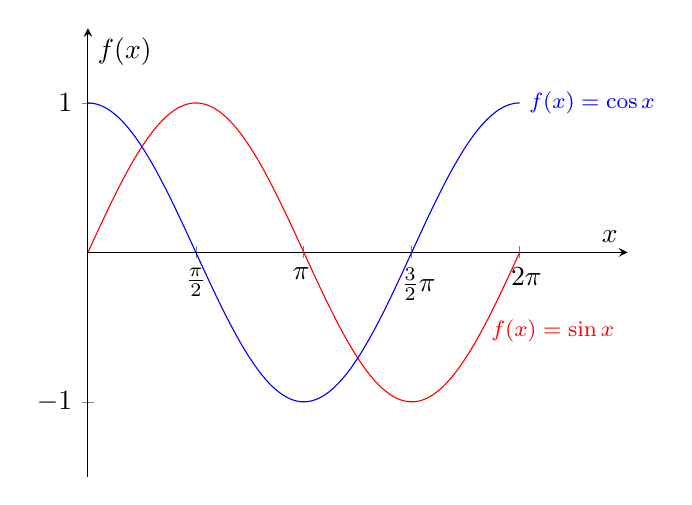
\begin{tikzpicture}
    \begin{axis}[
     clip=false,
     xmin=0,xmax=2.5*pi,
     xlabel= $x$,
     ylabel=$f(x)$,
     ymin=-1.5,ymax=1.5,
     axis lines=middle,
     %axis x line=middle,
     %axis y line=left,
     %axis x line=middle,
     xtick={0,1.57,3.14,4.71,6.28},
     xticklabels={$0$, $\frac{\pi}{2}$,$\pi\,$,$\,\,\,\frac{3}{2}\pi$,$\,\,\,2\pi$},
     %xticklabel style={anchor=north west}
     ]
      \addplot[domain=0:2*pi,samples=200,red]{sin(deg(x))}
                                node[right,pos=0.9,font=\footnotesize]{$f(x)=\sin x$};
      \addplot[domain=0:2*pi,samples=200,blue]{cos(deg(x))}
                                node[right,pos=1,font=\footnotesize]{$f(x)=\cos x$};
    \end{axis}
\end{tikzpicture}

            \caption{There is not difference at all!}
        \end{figure}
       \end{minipage}
    \end{center}

\end{frame}

\begin{frame}{3.2. Warps (Frequency $v$)}

    \begin{center}
        \begin{minipage}{.8\textwidth}\rmfamily
        \begin{figure}
            \begin{tabular}{ccc}
                  \subfloat[$v =  2$]{\includegraphics[width=2.666cm]{images/warps/clock_fr_2.png}} 
                & \subfloat[$v =  5$]{\includegraphics[width=2.666cm]{images/warps/clock_fr_5.png}}
                & \subfloat[$v = 10$]{\includegraphics[width=2.666cm]{images/warps/clock_fr_10.png}}\\
                  \subfloat[$v = 15$]{\includegraphics[width=2.666cm]{images/warps/clock_fr_15.png}}
                & \subfloat[$v = 20$]{\includegraphics[width=2.666cm]{images/warps/clock_fr_20.png}}
                & \subfloat[$v = 30$]{\includegraphics[width=2.666cm]{images/warps/clock_fr_30.png}}
            \end{tabular}
        \end{figure}
       \end{minipage}
    \end{center}

\end{frame}

\begin{frame}{3.2. First combination}

    \begin{center}
        \begin{minipage}{.4\textwidth}\rmfamily
            \begin{figure}
                \includegraphics[width=4.666cm]{images/warps/combination_1.png}
            \end{figure}
            \begin{itemize}
                \item $\alpha_x = 10$, $\alpha_y = 15$
                \item $\phi_x = 10.5$, $\phi_y = 1$
                \item $v = x$
            \end{itemize}
       \end{minipage}
    \end{center}

\end{frame}

\begin{frame}{3.2. Second combination}

    \begin{center}
        \begin{minipage}{.8\textwidth}\rmfamily
            \begin{figure}
                \includegraphics[width=4.666cm]{images/warps/combination_2.png}
            \end{figure}
            \begin{itemize}
                \item $\alpha_x = 100$, $\alpha_y = 0$
                \item $\phi_x = 1$, $\phi_y = 0$
                \item $v = 4.66$, (infinite posibilities)
            \end{itemize}
       \end{minipage}
    \end{center}

\end{frame}

\section{Cylinder anamorphosis}
\begin{frame}{3.3. Cylinder anamorphosis}
    \begin{center}

        \begin{figure}
            \subfloat[Original]{\includegraphics[height=2.000cm]{images/original.png}}
        \end{figure}

        \begin{figure}
            \begin{tabular}{ccc}
                \subfloat[Radius 0]{\includegraphics[width=2.666cm]{images/zero.png}} 
                & \subfloat[Radius 3]{\includegraphics[width=2.666cm]{images/donuts_1.png}}
                & \subfloat[Radius 6]{\includegraphics[width=2.666cm]{images/donuts_2.png}}\\
            \end{tabular}
        \end{figure}

    \end{center}
\end{frame}

\begin{frame}{3.3. Cylinder anamorphosis}

    \begin{center}

        \begin{figure}
            \begin{tabular}{ccc}
                \subfloat[Radius 0]{\includegraphics[width=2.666cm]{images/czero.png}} 
                & \subfloat[Radius 3]{\includegraphics[width=2.666cm]{images/cdonuts_1.png}}
                & \subfloat[Radius 6]{\includegraphics[width=2.666cm]{images/cdonuts_2.png}}\\
            \end{tabular}
        \end{figure}

    \end{center}
\end{frame}

\section{Transformation of coordinates}

\begin{frame}{Polar coordinates}

\begin{center}
  \begin{tikzpicture}
    %Circles 
    \foreach \r in {1, 2,...,7}
      \draw[SteelBlue3, thick] (0,0) circle (\r);    
    \foreach \r in {0.5, 1.5,...,7}
      \draw[Azure4, thin] (0,0) circle (\r);
    %1° Rays
    \foreach \a in {0, 1,...,359}
      \draw[Azure4] (\a:7.7) -- (\a:8);
    %5° Rays
    \foreach \a in {0, 5,...,359}
      \draw[Azure4] (\a:7.5) -- (\a:8);      
    %15° Rays
    \foreach \a in {0, 15,...,359}
      \draw[thick,Azure4] (\a:1) -- (\a:8); 
    %30° Rays
    \foreach \a in {0, 30,...,359}
      \draw[thick,Azure4] (0, 0) -- (\a:8);
    %Radius labels (background filled white)
    \foreach \r in {1, 2,...,7}
      \draw (\r,0) node[inner sep=1pt,below=3pt,rectangle,fill=white] {$\r$};
    %Main rays
    \foreach \a in {0, 90,...,359}
      \draw[very thick] (0, 0) -- (\a:8);
    %Angle labels  
    \foreach \a in {0, 15,...,359}
      \draw (\a: 8.5) node {$\a^\circ$};
    %Central point
    \draw[fill=red] (0,0) circle(0.7mm);
  \end{tikzpicture}
\end{center}
\end{frame}

\begin{frame}{3.4. Transformation of coordinates}
    \begin{center}
        \begin{minipage}{.8\textwidth}\rmfamily
        \begin{figure}
            \begin{tabular}{ccc}
                  \subfloat[$r,\varphi$]{\includegraphics[width=2.666cm]{images/one_.png}} 
                & \subfloat[$\varphi$-axis blurred]{\includegraphics[width=2.666cm]{images/two_.png}}
                & \subfloat[new $x, y$]{\includegraphics[width=2.666cm]{images/fin_.png}}
            \end{tabular}
        \end{figure}
       \end{minipage}
    \end{center}
\end{frame}

\section{Perspective Mapping Between Quadrilaterals}
\begin{frame}{3.5. Perspective Mapping Between Quadrilaterals}
    \begin{itemize}
        \item What is the main problem?
        \item Calculate the transformation matrix so our image fits inside the poster
        \item The solution is use \textit{homography}.
    \end{itemize}
\end{frame}
\begin{frame}{3.5. Perspective Mapping Between Quadrilaterals}
    \begin{itemize}
        \item What is homography?
        \item A homography is a transformation (a $3\times3$ matrix) that maps the points in one image to the corresponding points in the other image.
    \end{itemize}
\end{frame}
\begin{frame}{How to do it?}
    \begin{itemize}
        \item 1. Load images
    \end{itemize}

        \begin{figure}
                \includegraphics[width=4.666cm]{images/clock.jpg}
                \includegraphics[width=4.666cm]{images/isle.jpg}
        \end{figure}

\end{frame}
\begin{frame}{How to do it?}
    \begin{itemize}
        \item 2. Define the corners where to put the small image
        \item 3. Calculate \textit{homography} between source and destination points
        \item 4. Generate warped small image in an image size like the destination one
    \end{itemize}
    \begin{figure}
        \includegraphics[width=4.666cm]{images/clock-warped.jpg}
    \end{figure}
\end{frame}

\begin{frame}{How to do it?}
    \begin{itemize}
        \item 5. Black out polygonal area in destination image.
        \begin{figure}
            \includegraphics[width=4.666cm]{images/isle-black.PNG}
        \end{figure}
    \end{itemize}
\end{frame}

\begin{frame}{Results}
    \begin{itemize}
        \item 6. Add warped source image to destination image.
        \begin{figure}
                \includegraphics[width=4.666cm]{images/task5-result.PNG}
            \end{figure}
    \end{itemize}
\end{frame}

\begin{frame}{Results}
 \begin{figure}
             \begin{tabular}{cc}
                {\includegraphics[width=5.666cm]{images/times-square.jpg}} 
              & {\includegraphics[width=5.666cm]{images/task5-extra-2.PNG}}
            \end{tabular}
             \end{figure}
\end{frame}

\end{document}
